\documentclass[11pt]{article}
\usepackage[a4paper,margin=2.5cm]{geometry}
\usepackage[T1]{fontenc}
\usepackage{lmodern}
\usepackage{amsmath,amssymb}
\usepackage{graphicx}
\usepackage{booktabs}
\usepackage{siunitx}
\usepackage[hidelinks]{hyperref}
\usepackage{caption}
\usepackage{placeins}
\captionsetup{font=small,labelfont=bf}

% Every number below that comes from a simulation is a macro defined in results.tex,
% which scripts/make_figures.py writes from the data in ../data/.
% Written by scripts/make_figures.py from data/ - do not edit by hand
\newcommand{\BozicInside}{40}
\newcommand{\BozicLesions}{4{,}000}
\newcommand{\BozicMaxDiff}{0.009}
\newcommand{\BozicNTwentyBurden}{\num{1.29e+09}}
\newcommand{\BozicNTwentyEq}{0.821}
\newcommand{\BozicNoCross}{0.999}
\newcommand{\BozicOneCross}{0.26}
\newcommand{\BozicPatientReps}{1{,}000}
\newcommand{\BozicPatients}{22}
\newcommand{\BozicPatientsMatch}{21}
\newcommand{\BozicPatientsSimInside}{42}
\newcommand{\BozicPatientsSimTotal}{44}
\newcommand{\BozicPoints}{40}
\newcommand{\BozicTwoStepDev}{8--39\,\%}
\newcommand{\BozicTwoStepFormula}{0.0036}
\newcommand{\BozicTwoStepSim}{0.0029 [0.0022, 0.0037]}
\newcommand{\CAEdgeTouches}{0}
\newcommand{\CAParadoxHigh}{167{,}773}
\newcommand{\CAParadoxLow}{56{,}922}
\newcommand{\CAPmMatch}{0.61}
\newcommand{\CAQuiescent}{71\,\%}
\newcommand{\CASizeCellWidths}{60{,}692}
\newcommand{\CASizeLiteral}{328{,}155}
\newcommand{\CAStemRatio}{12}
\newcommand{\CATumours}{32}


\title{Independent replication of two stochastic models of cancer:\\
resistance to combination therapy (Bozic et al., 2013) and\\
cancer stem cell driven tumour growth (Enderling et al., 2009)}
\author{Bertrand Mercier des Rochettes\\[2pt]
\small Quantum Proteins AI, Cergy-Pontoise, France\\
\small ORCID \href{https://orcid.org/0000-0002-1145-1881}{0000-0002-1145-1881},
\href{mailto:contact@quantum-proteins.ai}{contact@quantum-proteins.ai}}
\date{Draft, \today}

\begin{document}
\maketitle

\begin{abstract}
Computational models of cancer are often used beyond the paper that introduced them, yet
they are rarely re-implemented independently. We re-implemented, from the published
descriptions only, two widely cited stochastic models and compared our results with the
published ones. (i) The multitype branching process of Bozic et al.\ (eLife 2013) for the
evolution of resistance to targeted combination therapy: at the parameters of their
Figure~3, the analytic probability of eradication (their equation~1) lies inside the 95\,\%
confidence interval of our simulation at \BozicInside{} of \BozicPoints{} points, for mono
and dual therapy and up to two cross-resistance mutations. A secondary approximation, the
probability that two-step resistance is present at detection, is \BozicTwoStepDev{} lower
in simulation than the formula predicts, with tau-leaping or exact event-by-event simulation
alike. Their patient-level failure probabilities (Table~1) are reproduced for
\BozicPatientsMatch{} of \BozicPatients{} patients; for the remaining one, the paper's table and
supplementary data disagree. (ii) The cancer stem cell cellular
automaton of Enderling et al.\ (Cancer Res 2009), as specified by Poleszczuk \& Enderling
(2014): we reproduce the central ``paradox'' that a higher spontaneous death rate of
non-stem cells produces larger tumours (\CAParadoxLow{} cells at $\alpha=0$ versus
\CAParadoxHigh{} at $\alpha=0.2$ after 180~days, with \CAStemRatio{}-fold more stem
cells) and the reported fraction of cells without free space (\CAQuiescent{}). The
published tumour size (about 140{,}000 cells at 180 days) is not reproduced with the
migration rule read in cell widths (\CASizeCellWidths{} cells) and is exceeded with the
other possible reading (\CASizeLiteral{} cells); the original code is no longer available.
All code, data and scripts are open, and each result can be regenerated from a seed.
\end{abstract}

\section{Introduction}
Replicating a computational result means obtaining it again with an independent
implementation written from the published description \cite{rescience}. It tests both the
result and the description: whatever a reader cannot implement from the paper is, in
practice, not part of the model. Stochastic models of cancer evolution and growth are good
candidates, because they are reused in later studies and their results depend on details
(update order, event timing, boundary rules) that methods sections tend to compress.

We replicated two such models. Bozic et al.\ \cite{bozic2013} modelled the evolution of
resistance in melanoma lesions under targeted therapy with a multitype birth--death process
and derived closed-form probabilities of eradication under one or two drugs; their key
conclusion is that a single mutation conferring cross-resistance to both drugs can prevent
any hope of cure by dual therapy. Enderling et al.\ \cite{enderling2009} introduced a
cellular automaton of cancer stem cells and their non-stem progeny and reported that
increasing the death rate of non-stem cells can paradoxically accelerate long-term tumour
growth; Poleszczuk \& Enderling \cite{poleszczuk2014} later gave a compact specification of
the model with explicit parameter values, which we used.

\section{Methods}

\subsection{Resistance to combination therapy}
\paragraph{Model.} As in \cite{bozic2013} (Materials and methods): four cell types 00, 10,
01, 11 (1 = resistant to drug 1 or drug 2). Before treatment, every cell divides at rate
$b$ and dies at rate $d$; the offspring of a 00 cell is of type 10, 01 or 11 with
probabilities $u n_1$, $u n_2$, $u n_{12}$; that of a 10 cell is 11 with probability
$u(n_2+n_{12})$ (symmetrically for 01). The lesion grows from one fully sensitive cell
until it has $M$ cells; treatment then starts, during which cells sensitive to at least one
drug in use divide at $b'$ and die at $d'$, and fully resistant cells keep $b$ and $d$.
Parameters (their Figure~3): $b=0.14$, $d=0.13$, $d'=0.17$, $b'=b$ (per day), $u=10^{-9}$,
$n_1=n_2=50$, $n_{12}\in\{0,1,2\}$. For monotherapy, types sensitive to drug 1 (00, 01)
are treated.

\paragraph{Simulation.} Like the authors, we use a hybrid scheme: a cell type with fewer than
$K=1000$ cells evolves stochastically and larger ones deterministically, new mutants
arising as Poisson events \cite{bozic2013}. Where the authors simulate small populations
event by event, we advance them in steps of $\Delta t=0.1$~day with Poisson numbers of
births, deaths and mutant offspring (tau-leaping; $b\,\Delta t = 0.014$). A lesion whose
founding lineage dies out before reaching $M$ is restarted. After the start of treatment a
lesion is eradicated when no cell is left, and has failed when a resistant type reaches
$10^5$ cells (its extinction probability is then $(d/b)^{10^5}\approx 0$). Each lesion uses
its own random stream (xoshiro256**, seeded from the run seed and the lesion index), so
results do not depend on the number of threads. \BozicLesions{} lesions per parameter
point.

\paragraph{Comparison.} We compare the simulated probability of eradication, with its
Wilson 95\,\% interval, with equation~(1) of \cite{bozic2013},
$p_{\mathrm{erad}} = p_1^{\uparrow} p_1^{\downarrow} p_2^{\uparrow} p_2^{\downarrow}$, and the
simulated fraction of lesions in which fully resistant cells are present at the start of
treatment with $p_{\mathrm{res}} = 1-p_1 p_2$ (their formulas before equation~1). The
formulas were transcribed from the article's MathML to avoid ambiguities of the rendered
text.

\subsection{Cancer stem cell cellular automaton}
\paragraph{Model.} As specified in \cite{poleszczuk2014}: a two-dimensional square lattice
(one cell per \SI{10}{\micro\meter} site), Moore neighbourhood. Stem cells are immortal with
unlimited proliferation; at division they produce another stem cell with probability
$p_s=0.1$ and otherwise a non-stem cell with proliferation capacity $\rho_{\max}=10$.
Non-stem cells divide at most $\rho_{\max}$ times (the capacity decreases at each division
and is inherited by the daughter). Cells need a free neighbouring site to divide or move;
cells without one are quiescent. Each hourly step, cells present at the start of the step
are updated once in random order: with probability $p_d=1/24$ a cell attempts to divide
(cell cycle 24~h), otherwise it migrates with probability $p_m$ to a free neighbour chosen
uniformly. Non-stem cells die with probability $\alpha$ at a division attempt, or when
their capacity is exhausted; we took this rule from the later methods chapter of the same
group \cite{poleszczuk2016}, because \cite{poleszczuk2014} does not say when death is
tested. One stem cell starts in the centre; 180 days.

\paragraph{Migration.} \cite{poleszczuk2014} gives the motility as
$\mu=\SI{100}{\micro\meter\per\day}$ and $p_m=\mu\,\Delta t$. Read in cell widths, this is
$p_m = 10/24$ per step; read literally in micrometres it exceeds one, i.e.\ a cell that does
not divide always tries to move ($p_m=1$). We report both.

\paragraph{Ensembles.} \CATumours{} tumours per death rate ($\alpha\in\{0,0.01,0.05,0.1,0.2,0.3\}$,
lattice $1000\times1000$, none reached the edge), 16 per migration probability.

\section{Results}

\subsection{Resistance: equation (1) is reproduced}
Figure~\ref{fig:bozic} shows the probability of eradication against the number of cells at
the start of treatment. Equation~(1) lies inside the simulation's 95\,\% interval at
\BozicInside{} of \BozicPoints{} points; the largest absolute difference is \BozicMaxDiff{}.
The paper's central result is reproduced: with one cross-resistance mutation
($n_{12}=1$) the probability of eradicating a lesion of $10^9$ cells falls from
\BozicNoCross{} to \BozicOneCross{}, and monotherapy fails above about $10^8$ cells.

The probability that resistance to both drugs is present at the start of treatment is also
reproduced when it arises in one step ($n_{12}\ge 1$), but not when it requires two
mutations ($n_{12}=0$, $M=10^9$): simulation \BozicTwoStepSim{}, formula \BozicTwoStepFormula{}
(Table~\ref{tab:twostep}). The difference persists with a five times smaller time step, with a
ten times higher stochastic threshold, and with exact event-by-event simulation of the small
populations, as the authors did, so it is not an artefact of our scheme; the formula for $p_2$ is marked as an approximation in \cite{bozic2013}, and the
probability of eradication, which depends on surviving resistant lineages rather than on
transient cells present at one instant, agrees.

Finally, the expected number of resistant cells at detection,
$X\approx M n_{12}\mu$, is not a useful check of a simulation: the distribution is
heavy-tailed (Luria--Delbr\"uck-like), and a large share of the mean comes from mutations
that occur while the lesion is still small, in a tiny fraction of lesions. Sample means of
$10^4$ lesions fall well below $X$ while the medians and the probability of resistance
agree.

\paragraph{Patients.} Bozic et al.\ estimated the probability that dual therapy fails in 22
patients with metastatic disease, as one minus the product of equation~(1) over all lesions,
using lesion sizes listed in their Supplementary file~2 (their Table~1). Recomputing it from
that file reproduces Table~1 within 0.0015 for \BozicPatientsMatch{} of \BozicPatients{} patients
(Table~\ref{tab:patients}). Simulating every lesion (\BozicPatientReps{} replicates per patient)
gives failure probabilities consistent with equation~(1): the formula lies inside the
simulation's 95\,\% interval in \BozicPatientsSimInside{} of \BozicPatientsSimTotal{} cases.
Patient N20 is the exception to the first comparison: its three lesions in Supplementary
file~2 total \BozicNTwentyBurden{} cells, giving a failure probability of \BozicNTwentyEq{} with one
cross-resistance mutation, whereas Table~1 lists a burden of $1.6\times10^9$ cells and 0.881, which
is what equation~(1) gives for $1.6\times10^9$ cells. The two sources of the paper disagree for
this patient (a lesion missing from the supplementary file, or a typographical error); the
conclusion is unaffected.

\begin{table}[htbp]
\centering\scriptsize
\caption{Probability that dual therapy fails, per patient (lesion sizes from Supplementary
file~2 of \cite{bozic2013}; simulation: \BozicPatientReps{} replicates per patient). Monotherapy fails
with probability 1 in all patients in Table~1, equation~(1) and simulation.}
\label{tab:patients}
\begin{tabular}{lrr|rrr|rrr}
\toprule
 & & & \multicolumn{3}{c|}{dual, $n_{12}=1$} & \multicolumn{3}{c}{dual, $n_{12}=0$} \\
patient & lesions & cells & Table 1 & eq.~(1) & simulated & Table 1 & eq.~(1) & simulated \\
\midrule
N1 & 18 & \num{2.6e+11} & 1.000 & 1.000 & 1.000 & 0.283 & 0.283 & 0.258 \\
N2 & 25 & \num{2.3e+11} & 1.000 & 1.000 & 1.000 & 0.260 & 0.260 & 0.256 \\
N3 & 26 & \num{1.7e+11} & 1.000 & 1.000 & 1.000 & 0.203 & 0.203 & 0.182 \\
N4 & 30 & \num{1.4e+11} & 1.000 & 1.000 & 1.000 & 0.172 & 0.172 & 0.175 \\
N5 & 21 & \num{1e+11} & 1.000 & 1.000 & 1.000 & 0.128 & 0.128 & 0.119 \\
N6 & 8 & \num{9.8e+10} & 1.000 & 1.000 & 1.000 & 0.120 & 0.120 & 0.118 \\
N7 & 25 & \num{9.1e+10} & 1.000 & 1.000 & 1.000 & 0.112 & 0.112 & 0.097 \\
N8 & 8 & \num{7.4e+10} & 1.000 & 1.000 & 1.000 & 0.092 & 0.091 & 0.093 \\
N9 & 23 & \num{6.4e+10} & 1.000 & 1.000 & 1.000 & 0.080 & 0.080 & 0.071 \\
N10 & 5 & \num{5.5e+10} & 1.000 & 1.000 & 1.000 & 0.069 & 0.069 & 0.079 \\
N11 & 14 & \num{5.4e+10} & 1.000 & 1.000 & 1.000 & 0.068 & 0.068 & 0.058 \\
N12 & 23 & \num{4.8e+10} & 1.000 & 1.000 & 1.000 & 0.061 & 0.061 & 0.071 \\
N13 & 9 & \num{4.1e+10} & 1.000 & 1.000 & 1.000 & 0.052 & 0.052 & 0.055 \\
N14 & 13 & \num{4.1e+10} & 1.000 & 1.000 & 1.000 & 0.051 & 0.051 & 0.047 \\
N15 & 8 & \num{3.4e+10} & 1.000 & 1.000 & 1.000 & 0.042 & 0.043 & 0.027 \\
N16 & 7 & \num{2.2e+10} & 1.000 & 1.000 & 1.000 & 0.028 & 0.028 & 0.029 \\
N17 & 10 & \num{2.1e+10} & 1.000 & 1.000 & 1.000 & 0.027 & 0.027 & 0.024 \\
N18 & 4 & \num{2e+10} & 1.000 & 1.000 & 1.000 & 0.026 & 0.026 & 0.018 \\
N19 & 9 & \num{1.8e+10} & 1.000 & 1.000 & 1.000 & 0.023 & 0.023 & 0.018 \\
N20 & 3 & \num{1.3e+09} & 0.881 & 0.821 & 0.825 & 0.002 & 0.002 & 0.002 \\
N21 & 21 & \num{1.3e+09} & 0.828 & 0.828 & 0.811 & 0.002 & 0.002 & 0.001 \\
N22 & 1 & \num{8.5e+08} & 0.677 & 0.677 & 0.709 & 0.001 & 0.001 & 0.001 \\
\bottomrule
\end{tabular}

\end{table}

\begin{figure}[t]
\centering
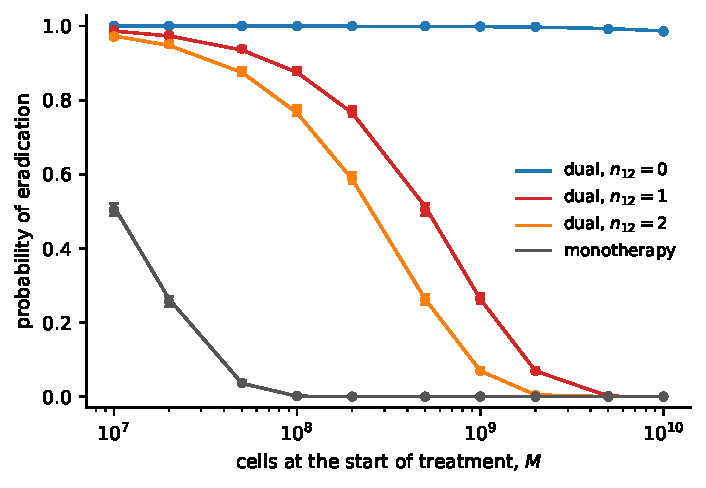
\includegraphics[width=0.8\linewidth]{../figures/bozic_eradication.pdf}
\caption{Probability of eradicating a lesion of $M$ cells (parameters of Figure~3 of
\cite{bozic2013}). Points: simulation (\BozicLesions{} lesions each, 95\,\% Wilson
intervals); lines: equation~(1) of \cite{bozic2013}.}
\label{fig:bozic}
\end{figure}

\begin{table}[htbp]
\centering\small
\caption{Two-step resistance present at the start of treatment (dual therapy, $n_{12}=0$,
$M=10^9$, 20{,}000 lesions each).}
\label{tab:twostep}
\begin{tabular}{lrrrr}
\toprule
small populations & $\Delta t$ (day) & threshold $K$ & simulated (95\,\% CI) & formula $1-p_1p_2$ \\
\midrule
tau-leaping & 0.1 & 1{,}000 & 0.0029 [0.0022, 0.0037] & 0.0036 \\
tau-leaping & 0.1 & 10{,}000 & 0.0033 [0.0026, 0.0042] & 0.0036 \\
tau-leaping & 0.02 & 1{,}000 & 0.0022 [0.0016, 0.0030] & 0.0036 \\
exact events & 0.1 & 1{,}000 & 0.0023 [0.0017, 0.0031] & 0.0036 \\
\bottomrule
\end{tabular}

\end{table}

\FloatBarrier
\subsection{Cellular automaton: the paradox is reproduced, the tumour size is not}
Table~\ref{tab:paradox} and Figure~\ref{fig:ca} show tumours after 180 days for increasing
death rates of non-stem cells. Tumours grow larger as $\alpha$ increases from 0 to 0.2
(\CAParadoxLow{} to \CAParadoxHigh{} cells), with many more stem cells, as reported in
\cite{enderling2009}: dying non-stem cells free space in which stem cells can divide. More than
70\,\% of cells have no free neighbour (\CAQuiescent{} at $\alpha=0.01$), as reported in
\cite{poleszczuk2014}.

The published size, about 140{,}000 cells after 180 days at $\alpha=0.01$
\cite{poleszczuk2014}, is not reproduced with $p_m=10/24$ (\CASizeCellWidths{} cells, mean
of \CATumours{}) and is exceeded with $p_m=1$ (\CASizeLiteral{} cells, 16 tumours).
Figure~\ref{fig:migration} shows that the final size grows steeply with $p_m$ and that the
published size corresponds to $p_m\approx\CAPmMatch{}$ in our implementation. The
original code, announced in \cite{poleszczuk2014}, could not be found; the specification
leaves the migration rule, and the timing of death, open enough to change the tumour size
by a factor of five.

\begin{table}[htbp]
\centering\small
\caption{Tumours after 180 days ($p_m=10/24$, \CATumours{} tumours each; mean $\pm$ standard error).}
\label{tab:paradox}
\begin{tabular}{rrrr}
\toprule
$\alpha$ & cells & stem cells & without free neighbour \\
\midrule
0 & 56{,}922 $\pm$ 3{,}068 & 150 $\pm$ 9 & 70.2\,\% \\
0.01 & 60{,}692 $\pm$ 2{,}604 & 173 $\pm$ 7 & 71.3\,\% \\
0.05 & 85{,}645 $\pm$ 3{,}529 & 305 $\pm$ 13 & 75.6\,\% \\
0.1 & 116{,}699 $\pm$ 3{,}967 & 571 $\pm$ 19 & 78.1\,\% \\
0.2 & 167{,}773 $\pm$ 4{,}932 & 1811 $\pm$ 53 & 83.1\,\% \\
0.3 & 179{,}227 $\pm$ 4{,}500 & 4794 $\pm$ 122 & 84.7\,\% \\
\bottomrule
\end{tabular}

\end{table}

\begin{figure}[t]
\centering
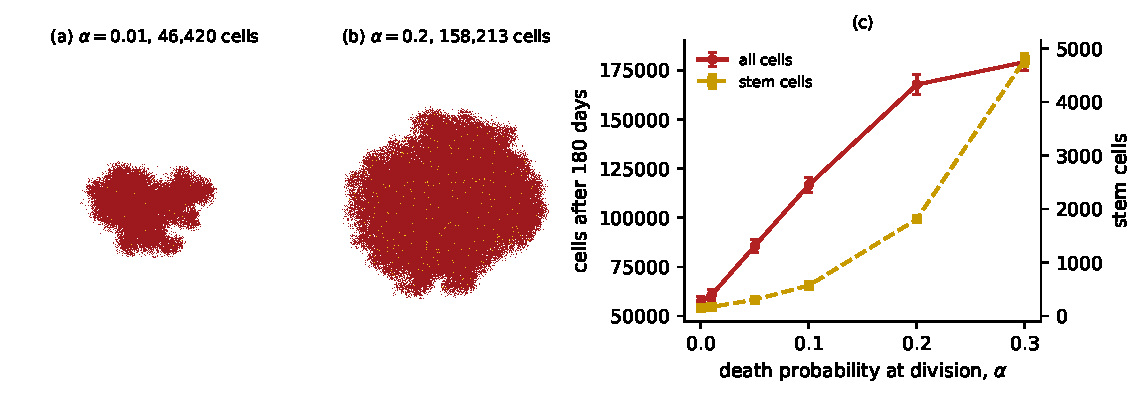
\includegraphics[width=\linewidth]{../figures/ca_paradox.pdf}
\caption{Cancer stem cell automaton after 180 days. (a, b) One tumour at $\alpha=0.01$ and
$\alpha=0.2$ (same seed; stem cells in yellow, each panel \SI{7}{\milli\meter} wide).
(c) Final number of cells and of stem cells against $\alpha$ (mean $\pm$ s.e.,
\CATumours{} tumours each).}
\label{fig:ca}
\end{figure}

\begin{figure}[t]
\centering
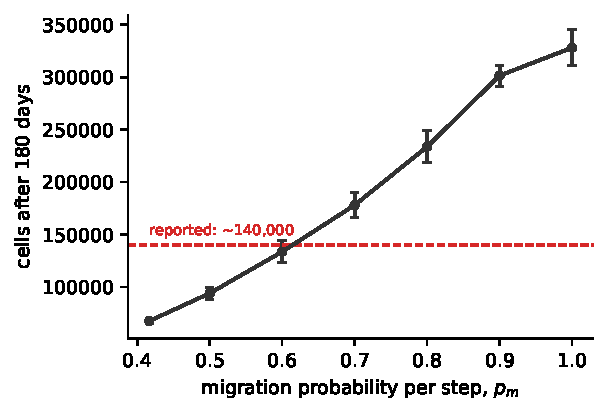
\includegraphics[width=0.6\linewidth]{../figures/ca_migration.pdf}
\caption{Tumour size after 180 days against the migration probability per step ($\alpha=0.01$,
16 tumours each, mean $\pm$ s.e.). Dashed: about 140{,}000 cells reported in
\cite{poleszczuk2014}. The two readings of $\mu=\SI{100}{\micro\meter\per\day}$ are
$p_m=10/24$ (cell widths) and $p_m=1$.}
\label{fig:migration}
\end{figure}

\FloatBarrier
\section{Discussion}
Both models are reproducible in the sense that matters most: their main published
conclusions follow from an independent implementation written from the papers. The
replication also shows where the descriptions are incomplete. For the resistance model, one
approximate formula should not be used as a quantitative check of a simulation (two-step
resistance present at detection), and the mean number of resistant cells is a poor
statistic for a heavy-tailed distribution. For the cellular automaton, the tumour size
depends strongly on two rules that are not fully specified (the migration probability and
when spontaneous death is tested); quantitative comparisons with this model therefore need
the rule stated explicitly, and we report ours.

\paragraph{Limitations.} Our main runs use tau-leaping where the authors simulated small
populations event by event; the agreement of the eradication probabilities, and the
identical two-step result of our exact event-by-event option (Table~\ref{tab:twostep}),
suggest the difference is negligible. Our automaton reference uses a fixed lattice large enough
that no tumour reached the edge, not a dynamically growing domain. We did not have access
to the original code of either study.

\section*{Code and data availability}
All code, data and scripts: \url{https://github.com/quantumproteinsai/rescience-bozic2013-enderling2009} [archive DOI, to be added at submission].
The resistance simulation is \texttt{src/resistance/resistance\_core.h} (C++), the automaton
reference is \texttt{src/ca/ca\_reference.cpp}; \texttt{make all} rebuilds the programs,
regenerates every number and figure from fixed seeds and compiles this manuscript.

\section*{Use of AI assistance}
The software, simulations, analyses and the first draft of this manuscript were produced
with an AI coding assistant (Claude Opus 5.5, Anthropic, used through Claude Code), under
the direction of the author. The author defined the study, chose the models and the
comparisons, checked the results against the original publications, and revised the text.
The AI is not an author; the author takes full responsibility for the content. All code,
data and the scripts that generate every reported number are openly available, so the
results can be checked independently of how they were produced.

\begin{thebibliography}{9}
\bibitem{bozic2013} Bozic I, Reiter JG, Allen B, Antal T, Chatterjee K, Shah P, et al.
Evolutionary dynamics of cancer in response to targeted combination therapy. eLife.
2013;2:e00747. doi:10.7554/eLife.00747
\bibitem{enderling2009} Enderling H, Anderson ARA, Chaplain MAJ, Beheshti A, Hlatky L,
Hahnfeldt P. Paradoxical dependencies of tumor dormancy and progression on basic cell
kinetics. Cancer Research. 2009;69:8814--8821. doi:10.1158/0008-5472.CAN-09-2115
\bibitem{poleszczuk2014} Poleszczuk J, Enderling H. A high-performance cellular automaton
model of tumor growth with dynamically growing domains. Applied Mathematics.
2014;5:144--152. doi:10.4236/am.2014.51017
\bibitem{poleszczuk2016} Poleszczuk J, Macklin P, Enderling H. Agent-based modeling of
cancer stem cell driven solid tumor growth. Methods Mol Biol. 2016;1516:335--346.
doi:10.1007/7651\_2016\_346
\bibitem{rescience} Rougier NP, Hinsen K, Alexandre F, et al. Sustainable computational
science: the ReScience initiative. PeerJ Computer Science. 2017;3:e142.
doi:10.7717/peerj-cs.142
\end{thebibliography}

\end{document}
